\subsection{Computational search over the entire normalized smoothness domain}
\label{sec:consolidated-computation}
The numerical tasks of (i) reconstructing a smoothed trend, (ii)
computing its effective degrees of freedom or statistical criterion,
(iii) inverting the normalized smoothness coordinate
$s=S(\lambda)$, and (iv) finding a criterion-minimizing penalty
are different workloads. We therefore do not identify the solver
with the optimization algorithm or with the statistical criterion.
For each $1\le d<n$, put $r=n-d$ and let
$\delta_1,\ldots,\delta_r$ denote the positive eigenvalues of
$Q_d=D_d^\top D_d$. The normalized map is
\begin{equation}\label{eq:full-s-inverse}
s=S(\lambda)=\frac{1}{r}\sum_{j=1}^{r}
\frac{\lambda\delta_j}{1+\lambda\delta_j},
\qquad
S'(\lambda)=\frac1r\sum_{j=1}^{r}
\frac{\delta_j}{(1+\lambda\delta_j)^2}>0.
\end{equation}
The inverse $S^{-1}(s)$ is unique for $0<s<1$; the
\emph{exact} limits are $S^{-1}(0)=0$ and
$S^{-1}(1)=+\infty$. At a fixed difference order and
reference mean, minimizing any criterion $C(\lambda)$ on
the same domain is mathematically equivalent to minimizing
$C(S^{-1}(s))$, but the \emph{numerical} cost and the
sampled candidate locations can differ.

Our previously completed Windows workstation experiment,
archived independently from the present paper's empirical
examples, consists of \textbf{80,640 recorded search trials}.
The factors are seven implementations (fresh and cached dense
solves, general banded solves, dense and banded Cholesky,
symmetric eigendecomposition and SVD), five criteria
(CV, GCV, AICc, BIC and conditional Gaussian profile MLE),
$n\in\{24,48\}$, difference orders $d=0,\ldots,5$,
fixed $\mu\in\{0,0.15\}$, and one, three or eight
independent observation series, with cold and reusable
preparation. Two synthetic data seeds, seven timings per
configuration and a one-thread BLAS limit are reported.
The $S$ grid contains seventeen points, including the
exact endpoints and values up to $1-10^{-12}$.
Gaussian MLE for $d=0$ is reported as not applicable
under the adopted likelihood, and unstable extreme
finite-penalty scores are excluded from numerical-win
claims rather than silently dropped.

\begin{figure}[tbp]
\centering
\IfFileExists{figures/windows_full_s_workloads.pdf}{%
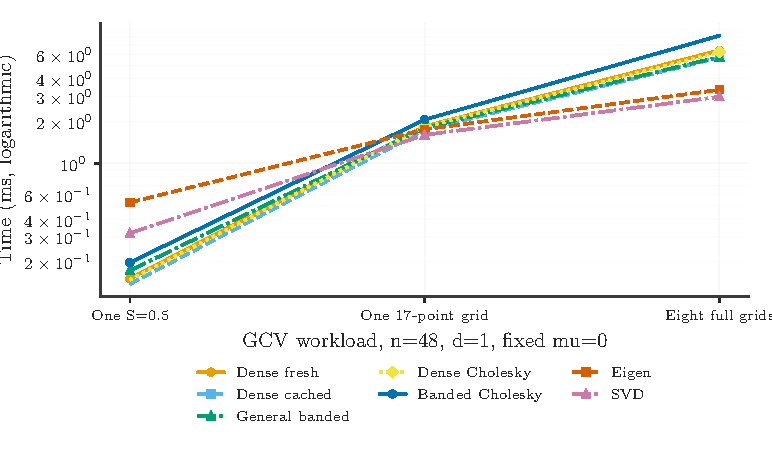
\includegraphics[width=\linewidth]{figures/windows_full_s_workloads.pdf}
}{\fbox{The verified Windows workload figure is generated by the supplied final VM runner.}}
\caption{Existing Windows author-run measurements for one
scalar GCV evaluation, a complete mapped-$S$ search and
repeated independent complete searches. Solver setup and
criterion work must be distinguished. The plot's numerical
validity filters, $n,d,\mu$, and hardware characteristics
are described in the archived study, not pooled with
hosted-Linux measurements.}
\label{fig:consolidated-windows-workloads}
\end{figure}

\begin{figure}[tbp]
\centering
\IfFileExists{figures/windows_full_s_grid_coordinates.pdf}{%
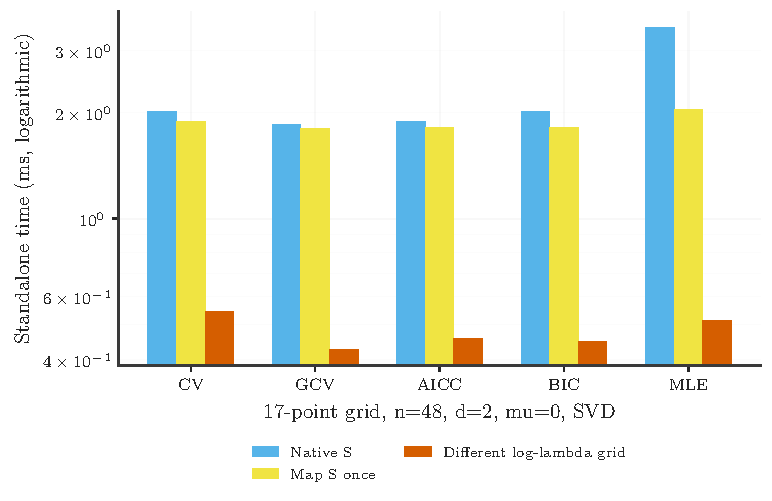
\includegraphics[width=\linewidth]{figures/windows_full_s_grid_coordinates.pdf}
}{\fbox{Verified mapped-grid plot generated by the final VM runner.}}
\caption{Same-candidate native-$S$ and once-mapped
$S\to\lambda$ finite-grid selections, contrasted with a
different log-$\lambda$ grid. The first two evaluate
\emph{identical} penalties and must select the same
criterion minimum. The independently spaced log-grid
has different interior candidates and cannot be treated
as a same-estimator speed comparison. A shared grid
inversion is charged once and may be amortized across
criteria and observations.}
\label{fig:consolidated-windows-coordinates}
\end{figure}

\begin{figure}[tbp]
\centering
\IfFileExists{figures/windows_full_s_bounded.pdf}{%
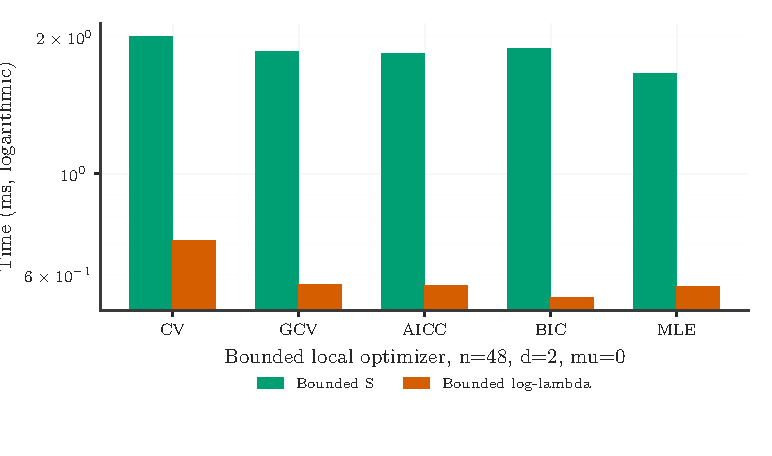
\includegraphics[width=\linewidth]{figures/windows_full_s_bounded.pdf}
}{\fbox{Verified bounded-search plot generated by the final VM runner.}}
\caption{Bounded \emph{local} continuous searches in
$s$ and $\log\lambda$ for the five criteria.
These have different evaluation locations and iteration
counts and are \emph{not} guaranteed global minimizers.
The corresponding measurement CSV, selection values,
hardware metadata and numerical validity checks are
part of the archived 80,640-trial study.}
\label{fig:consolidated-windows-bounded}
\end{figure}

A distinct repeated full-trend benchmark uses
\texttt{PreparedPLSSolver} with full SVD, symmetric
eigendecomposition of $Q_d$, and \emph{actual banded
Cholesky} (\texttt{cholesky\_banded} with
\texttt{cho\_solve\_banded}). This distinction matters:
our older general-banded competitor uses
\texttt{solve\_banded}, \emph{not} Cholesky.
The three methods produce the same fitted trends
within checked tolerances, while their relative speed
depends on $n$, order $d$, how many penalties are fitted,
and how much preprocessing can be reused.

\subsection{Paired uncertainty for full-trend solver comparisons}
\label{sec:solver-uncertainty}
To avoid interpreting timing noise as independent
statistical replication, the VM protocol randomizes the
order of the three solvers in every paired timing block,
feeds them the same observations and penalty grid, and
checks every fitted trend against the SVD reference
\emph{outside} the timed block. For each workload and
independently seeded synthetic observation series, the
primary outcome is the \emph{median end-to-end duration}
across repeated blocks (setup plus all full-trend fits).
The inferential unit is this per-data-seed summary;
neither the $M$ separate penalties nor the technical
timing repetitions are counted as independent samples.

For each of the three pairwise solver comparisons,
let $T_{a,i},T_{b,i}>0$ be the paired times for
independent data seed $i$. We estimate a geometric
mean runtime ratio
\[
 R_{a/b}=\exp\!\left(\frac1N
       \sum_{i=1}^N\log\frac{T_{a,i}}{T_{b,i}}\right).
\]
A ratio greater than one means implementation $b$
was faster on average for that \emph{specified} workload.
We construct 95\% pointwise percentile bootstrap intervals
by resampling the $N$ data seeds (not the timing blocks)
and test a zero mean paired log ratio by two-sided
sign-flip randomization, conditional on symmetry/
exchangeability of the paired differences.
Holm adjustment controls the specified family of
\emph{primary} comparisons across methods and workloads.
The bootstrap intervals themselves are \emph{not}
simultaneous or multiplicity-adjusted. A randomized
data seed does not eliminate systematic host timing bias;
all measurements still share one computer/session.

\IfFileExists{final_solver_inference_table.tex}{%
\begin{table}[tbp]\centering\footnotesize
\caption{Author Windows VM measured end-to-end
solver comparisons; geometric mean ratio
\emph{SVD divided by banded Cholesky}, with
95\% \emph{pointwise} bootstrap interval and
family-wise Holm-adjusted primary $p$ value.
Rows are a declared subset of the entire
workload family; all seed-level values and all
adjusted tests are published as CSV. The ratio
does not identify a universally fastest solver.}
\label{tab:final-solver-uncertainty}
\begin{tabular}{rrrrrr}
\toprule
$n$ & $d$ & $M$ & SVD / BChol & 95\% pointwise CI & Holm $p$ \\
\midrule
32 & 2 & 1 & 1.55 & [1.54, 1.57] & 0.00315 \\
32 & 2 & 16 & 0.68 & [0.68, 0.68] & 0.00315 \\
32 & 2 & 64 & 0.42 & [0.42, 0.42] & 0.00315 \\
96 & 2 & 1 & 4.22 & [4.20, 4.24] & 0.00315 \\
96 & 2 & 16 & 2.09 & [2.08, 2.10] & 0.00315 \\
96 & 2 & 64 & 0.97 & [0.96, 0.97] & 0.00315 \\
\bottomrule
\end{tabular}

\end{table}
}{%
\noindent\emph{Final author-VM solver inference table
not yet generated; run \texttt{run\_final\_vm\_study.py}.}\par
}

\IfFileExists{figures/final_solver_inference.pdf}{%
\begin{figure}[tbp]\centering
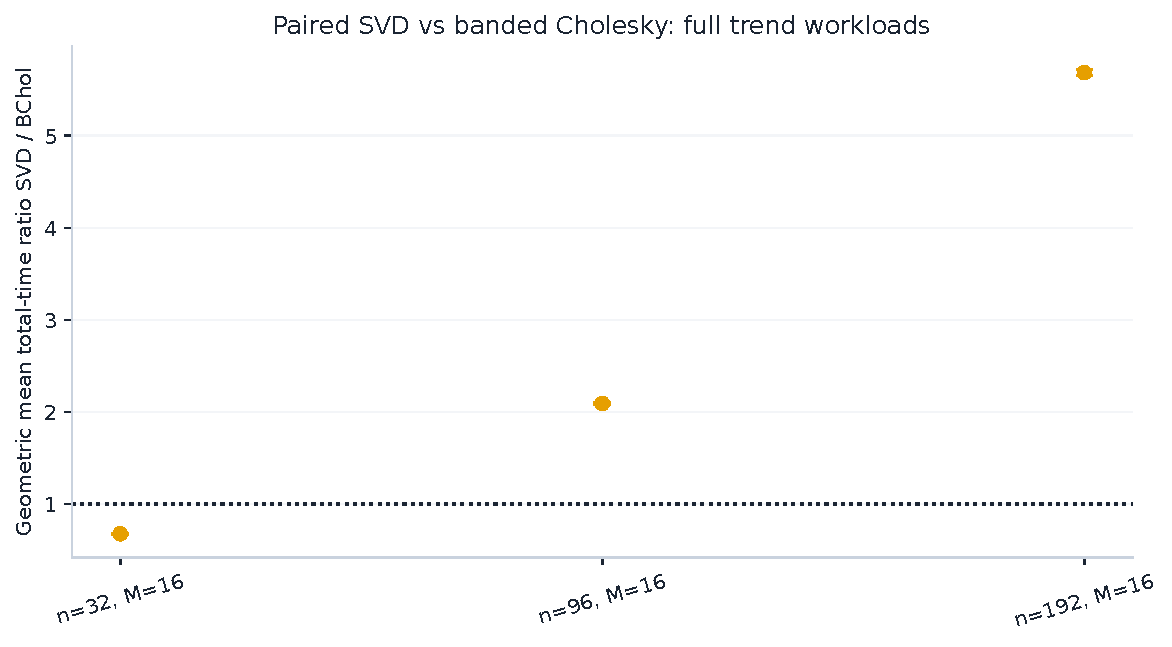
\includegraphics[width=.9\linewidth]{figures/final_solver_inference.pdf}
\caption{Paired full-trend solver runtime ratios for
the declared author-run workload subset. Error bars
are pointwise seed-bootstrap intervals; the horizontal
reference is equal elapsed time. The complete Holm
family, including eigendecomposition comparisons, is
in the archived statistical analysis.}
\label{fig:final-solver-uncertainty}
\end{figure}
}{}

\subsection{Numerical inversion: Brent, Newton, secant and bisection}
\label{sec:inversion-benchmark}
Inverting $S$ is required for a prescribed nontrivial
smoothness level. We benchmark four implemented
floating-point root methods applied in
$x=\log\lambda$: the bracketed Brent method,
bracket-safeguarded Newton, bracket-safeguarded secant,
and bisection. Their targets include $10^{-14}$,
$0.1$, $0.5$, $0.9$, $0.99$, and near-one values as
close as $1-10^{-14}$. The inverse accuracy comparison
is evaluated in the \emph{smaller probability tail}:
for $s>0.5$ the complement $1-S$ is evaluated directly,
rather than subtracting a value near one.
This matters in finite precision at both extremes.
Each method receives one identical, already prepared
spectral smoother for its $(n,d,s)$ case, and the order
of timed calls is randomized within each complete block.
Errors, failed convergence, derivative evaluations,
iteration counts, and latency are all retained,
including failed trials. For $d=0$ the positive
spectrum is scalar, so \emph{all} methods use the
same analytic inverse; these are not legitimate
numeric-root speed comparisons.

\IfFileExists{final_inversion_table.tex}{%
\begin{table}[tbp]\centering\footnotesize
\caption{Measured float64 inversion latencies at two
specified smoothness targets, including failures,
iterations and maximum relative tail error.
The target series length and difference order are
recorded in the machine-readable report. Medians
are taken over successful technical repetitions;
no bootstrap inference is assigned to dependent
timing calls within one host session.}
\label{tab:final-inverse-solvers}
\begin{tabular}{llrrrr}
\toprule
$S$ & Inversion method & Median $\mu$s & Fail / trials & Iterations & Max rel. tail error \\
\midrule
.5 & brentq & 91.50 & 0/35 & 10.0 & 1.8e-15 \\
.5 & newton & 88.30 & 0/35 & 5.0 & 2.2e-16 \\
.5 & secant & 157.70 & 0/35 & 24.0 & 1.1e-15 \\
.5 & bisect & 292.00 & 0/35 & 45.0 & 1.4e-13 \\
.99 & brentq & 93.70 & 0/35 & 11.0 & 3.3e-14 \\
.99 & newton & 118.60 & 0/35 & 8.0 & 0 \\
.99 & secant & 162.80 & 0/35 & 26.0 & 1.7e-13 \\
.99 & bisect & 282.00 & 0/35 & 45.0 & 7.7e-14 \\
\bottomrule
\end{tabular}

\end{table}
}{%
\noindent\emph{The inversion algorithm benchmark
requires the one-time author-VM run.}\par
}

\IfFileExists{figures/final_inversion_speed.pdf}{%
\begin{figure}[tbp]\centering
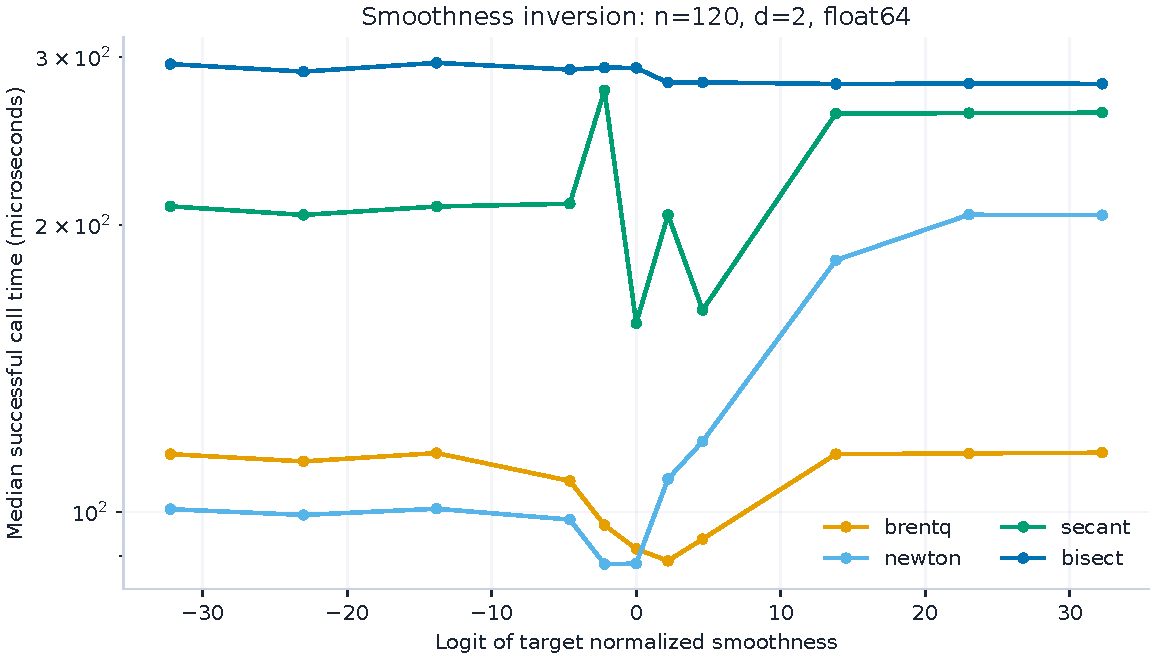
\includegraphics[width=.94\linewidth]{figures/final_inversion_speed.pdf}
\caption{Observed successful-call inversion time
across the normalized-smoothness range for
Brent, Newton, secant, and bisection. The
horizontal axis is logit$(S)$ so both endpoint
tails remain visible; method convergence failures
are reported in the source table. Fast but
numerically invalid results are not acceptable
substitutes for a correct inverse.}
\label{fig:final-inverse-solvers}
\end{figure}
}{}

\IfFileExists{final_computation_environment.tex}{%
\noindent\textit{Author-host study.} 
Paired solver: 20 independently seeded data replicates per workload, 5 randomized timing blocks per seed, 
21 workload configurations, 63 pairwise comparisons (63 eligible for Holm adjustment). Inversion: 
35 randomized timing blocks for each target, solver and finite-difference order, with 
0/13860 failed attempted inversions for non-analytic orders. Timing repeats on one machine are not independent samples; bootstrap CIs are pointwise, not familywise adjusted. All comparisons are conditional on the archived host, numerical precision, software and workload. 

}{%
\noindent\emph{The author-VM machine environment
and repeated study counts will be inserted
automatically after the benchmark.}\par
}

The new numerical inversion measurements answer a
different question from the complete parameter selection
timings: they include an \emph{already initialized}
spectral smoother and only one inversion call. That
preprocessing cost must be included before using such
microbenchmarks to choose between end-to-end search
policies. Nor do they establish a superior future
forecast or a new smoothing criterion. Source files,
raw paired measurements, failure records, statistical
tests, plots and machine information are archived
alongside the standalone manuscript under
\texttt{research/final\_vm/}; the existing 80,640-search
Windows source remains unchanged.
